\documentclass{../../text-style}

\texttitle{Лекция 11: Предметно-ориентированное проектирование, стратегические аспекты}
\author{Юрий Литвинов\\\small{y.litvinov@spbu.ru}}

\begin{document}

\maketitle
\thispagestyle{empty}

\section{Целостность модели}

Центральной идеей методологии предметно-ориентированного проектирования является единая модель предметной области и единый язык, что хорошо и правильно, но если над проектом работает сотня человек, это проблематично. Собрать всех на одной кухне, чтобы они могли оттачивать единый язык, физически невозможно, особенно если они на самом деле говорят на разных языках и сидят на разных континентах. В этой лекции речь пойдёт о том, как применять предметно-ориентированное проектирование к проектам, разрабатывающимся несколькими командами, о том, как вообще разрабатывать большие проекты, какие архитектурные проблемы при этом появляются и как их можно решать. Эта лекция по сути является кратким пересказом части IV книги <<Предметно-ориентированное проектирование (DDD). Структуризация сложных программных систем>>, Э. Эванс, и заканчивает рассказ о книге.

Итак, предметно-ориентированное проектирование в случае проекта, над которым работают несколько команд, сталкивается с проблемой того, что команды неизбежно имеют разные видения продукта. Эту проблему можно решать, 

\begin{itemize}
    \item либо поддерживая модель интегрированной --- но тогда затраты на поддержание её целостности будут слишком велики (в идеале --- все команды должны будут непосредственно общаться со всеми остальными, и каждое изменение в модели утверждаться остальными командами), при этом модель наверняка получится слишком общей, чтобы быть полезной;
    \item либо приняв ситуацию как должное и разрешив модели быть фрагментированной --- но тогда это неизбежно затруднит переиспользование кода в рамках проекта и интеграцию системы.
\end{itemize}

При этом бесконтрольное существование модели может привести к ошибкам, связанным с разным пониманием командами нюансов сущностей модели. Эрик Эванс приводил в книжке хороший пример, когда над системой работало несколько команд, и одной из них потребовалась абстракция для платежа клиента. Оказалось, что в коде уже был класс <<Платёж>>, разработанный другой командой, ну и, понятно, его решили переиспользовать. Парочки полей не хватало, одно называлось не совсем так, как надо, но ладно, в конце концов, какое имеет значение конкретное название. Однако система через пару дней начала внезапно падать, в модуле оплаты счетов субподрядчику, для которого изначально был разработан класс <<Платёж>>, в частности, на генерации налоговых отчётов. Стали разбираться, обнаружили в системе странные платежи, которые никто не вводил и которые не имели никакого смысла. Оказалось, что система крешилась из-за того, что у странных платежей не было заполнено поле <<необлагаемый процент>>, несмотря на то, что система требовала его заполнености и сама подставляла туда значение по умолчанию при создании платежа. Выяснилось, что это действительно были платежи клиентов, и для них действительно поле <<необлагаемый процент>> не имело смысла, поэтому просто не заполнялось. И эти платежи тоже попадали в вычисление налоговой отчётности (потому что они платежи же!) и всё падало.

Это выглядит как какая-то частная проблема, но корень зла тут вполне системный --- две команды использовали одну сущность в разных, хоть и похожих, смыслах. И не имели никакого механизма, позволявшего выявить заранее несоответствие значений, которые команды вкладывали в термин <<Платёж>>. Решением проблемы стало создание двух отдельных абстракций <<Платёж поставщику>> и <<Платёж клиента>> и договорённость более не мешать друг другу.

\subsection{Ограниченный контекст}

Командам из примера про <<Платёж>> могла бы помочь заранее достигнутая договорённость о границах их предметных областей и правилах переиспользования кода. В предметно-ориентированном проектировании для этого вводится понятие \textit{<<Ограниченный контекст>>}. Ограниченный контекст (Bounded context) --- это кусок предметной области (и, соответственно, реализующего её кода), в которой применима единая модель предметной области. Всё, что внутри ограниченного контекста, должно следовать этой единой модели, иметь единый язык и т.п., всё, что вне --- не должно делать никаких предположений о модели и не имеет право её без спроса переиспользовать. То есть, ограниченный контекст --- это что-то вроде атомарной области проекта, над которой работает одна команда (как клетка в живом организме, простите за банальную метафору). Разделение системы на ограниченные контексты обычно следует организационной структуре проекта, которая, в свою очередь, чаще всего следует высокоуровневой структуре системы. Например, в одном из проектов, в котором работал автор, по созданию средства автоматизированного реинжиниринга, была группа синтаксического анализа, группа извлечения бизнес-правил, группа генерации кода. Каждая группа имела собственный ограниченный контекст, свою терминологию и своё видение задачи, и интегрировалась с другими с помощью вполне определённых интерфейсов. Что происходило внутри, было делом каждой команды --- например, группа извлечения бизнес-правил занималась вообще какими-то магическими алгоритмами статического анализа программ, которые никто, кроме них, не понимал.

Внутри одного ограниченного контекста может работать довольно большое количество людей, между которыми также может возникнуть недопонимание, напряжение при попытке поддержания единого видения и т.п. Практика показывает, что 3-4 человека, тесно работая вместе, обычно могут договориться, но делить систему на ограниченные контексты по 3-4 человека оказывается непрактично. Поэтому в рамках ограниченного контекста практикуют \textit{<<непрерывную интеграцию>>} в её классическом понимании --- слияние изменений в основную ветку раз в несколько часов, постоянную (после каждого коммита) сборку и запуск юнит-тестов, обеспечение высокого тестового покрытия, непрерывное общение в рамках команды. Всё это позволяет быстро понять наличие проблем в понимании модели внутри ограниченного контекста и устранить их.

Для интеграции с другими ограниченными контекстами могут использоваться \textit{<<карты контекстов>>} (Context map). Карта контекстов фиксирует, как понятие из одной модели в рамках одного ограниченного контекста транслируется в понятие из другой модели из другого контекста. Карты трансляции обычно просто описываются на естественном языке (с применением терминов единых языков интегрируемых моделей), но могут и использоваться диаграммы такого примерно вида:

\begin{center}
    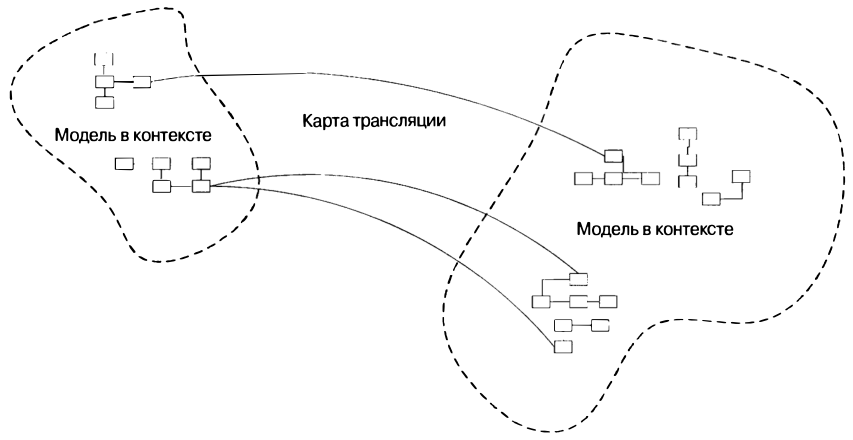
\includegraphics[width=0.8\textwidth]{contextMap.png}
\end{center}

Вот любимый Эриков Эвансом пример про сервис грузоперевозок, показывающий взаимосвязь ограниченных контекстов в рамках одной задачи: 

\begin{center}
    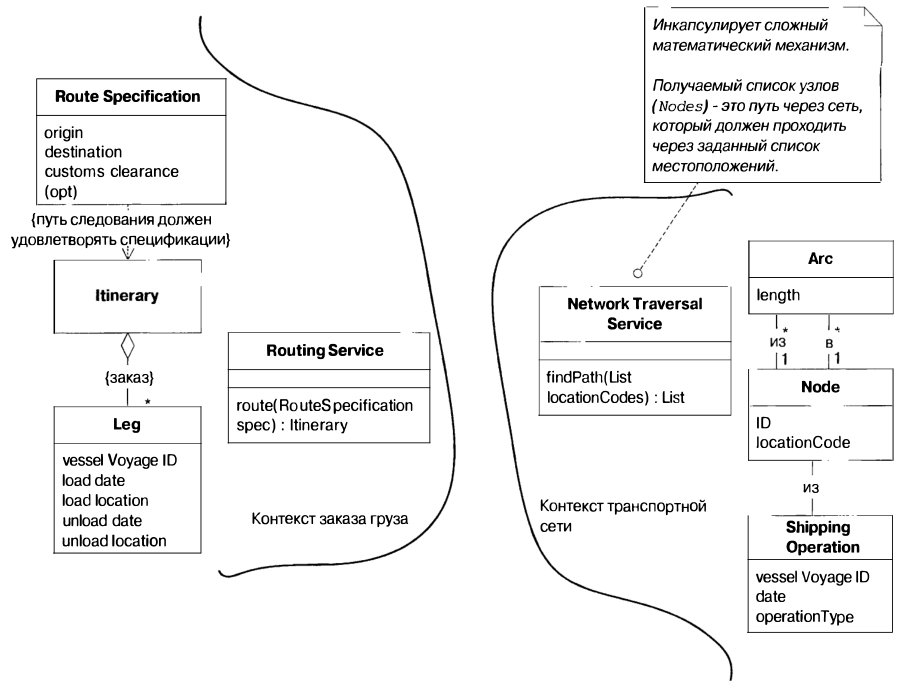
\includegraphics[width=0.9\textwidth]{contextBoundariesExample.png}
\end{center}

Есть команда, занимающаяся бизнес-логикой сервиса прокладки маршрута. Она оперирует понятиями <<Спецификация маршрута>>, <<Маршрут>>, <<Перевозка>> и использует <<Сервис прокладки маршрута>> для вызова кода второй команды, который собственно составляет маршрут перевозки между двумя точками. Вторая команда работает в терминах алгоритмов на графах, она ничего не знает и не хочет знать про перевозки, спецификации маршрута и конкретные корабли или поезда, везущие грузы. У них есть узлы и дуги с весами, узлы привязаны к координатам на местности и в узлах можно осуществлять погрузочно-разгрузочные операции над некоторыми абстрактными транспортными средствами, идентифицируемыми своим кодом. Это позволяет второй команде переиспользовать существующие библиотечные реализации графов и алгоритмов на них, не мучаясь со спецификой предметной области. Но это, естественно, требует определённых усилий на интеграцию, поскольку <<Сервис прокладки маршрута>> со стороны первой команды должен выполнять трансляцию в термины <<Сервиса поиска пути>> второй команды и обратно, и о том, как работают эти сервисы, команды должны чётко договориться. Зато всё, что находится за этими сервисами, может разрабатываться независимо. Что, конечно, приводит к дубликации кода, потому что Leg и Arc, по сути, выражают одно и то же понятие, но в данном случае это абсолютно осмысленно --- команды могут работать параллельно, не мешать друг другу и не мешать разные понятия в одну кучу.

\subsection{Паттерны интеграции контекстов}

Есть некоторые типичные ситуации, в которых возможны разные степени интеграции моделей предметной области и разные способы действий, необходимых, чтобы этой интеграции достичь и при этом не навредить разработке. Эванс в своей книге выделяет несколько подходов и даёт им имена (поэтому их можно рассматривать как что-то вроде паттернов интеграции контекстов). Выбор подхода, который стоит применять, зависит от конкретной ситуации и обстоятельств, скорее всего, не зависящих от команды. Поэтому стремиться к высокой интеграции контекстов не всегда стоит, и один из официальных подходов к интеграции --- это отказаться от интеграции вообще.

\subsubsection{Общее ядро}

Первый рассматриваемый здесь паттерн интеграции --- <<Общее ядро>> (Shared Kernel) --- предполагает наиболее тесную интеграцию, кроме объединения двух ограниченных контекстов в один. Такой подход предполагает выделение общей части двух ограниченных контекстов и совместную реализацию элементов модели оттуда:

\begin{center}
    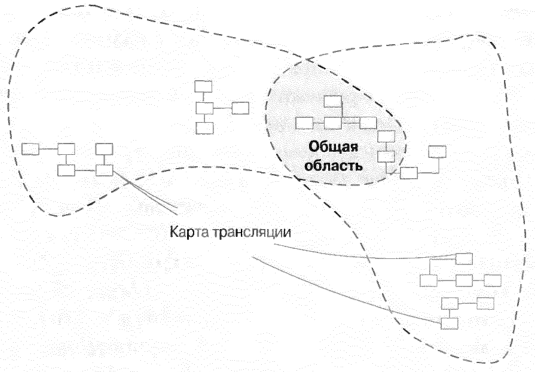
\includegraphics[width=0.7\textwidth]{sharedKernel.png}
\end{center}

Классы из общей области должны иметь строго одинаковый смысл во всех интегрируемых ограниченных контекстах. Обычно это либо какое-то общее ядро, определяющиек базовые понятия всей предметной области проекта, либо это могут быть какие-то классы с данными, которые используются для того, чтобы два ограниченных контекста могли легко и без дополнительных преобразований обмениваться информацией. При этом наличие общего ядра не отрицает применения карты трансляции к элементам модели, которые в общее ядро не попали.

Паттерн <<Общее ядро>> применим только в случае, если две команды могут непосредственно общаться друг с другом, находятся на одном уровне подчинения и не будут мешать друг другу. Классы из общего ядра можно менять только после согласования с обеими командами, так что это дело хлопотное, а необходимость избегать неправильного понимания сущностей и <<ересей>> в едином языке требует и постоянного неформального общения членов команд.

\subsubsection{Заказчик-поставщик}

Паттерн <<Заказчик-поставщик>> (Customer-Supplier) применяется, когда общение между командами затруднено и/или когда команщды находятся в подчинённом отношении друг к другу (не обязательно административно подчинённом, это может быть подчинение в смысле зависимостей между компонентами --- например, группа генерации кода может оказаться зависимой от группы синтаксического анализа, особенно если синтаксический анализ нужен не только генерации кода). Особенно паттерн актуален, когда команды имеют потенциально разный цикл релизов и ориентируются на разных конечных пользователей. <<Общее ядро>> в такой ситуации применять невозможно, поскольку попытка согласовать общее ядро может провалиться из-за близости релиза одной из команд, конфликтующих приоритетов или конфликтующих миропониманий. Тогда одна из команд рискует оказаться заблокированной.

Чтобы этого избежать, следует явно зафиксировать отношения между командами. Одна из команд выступает в роли заказчика (одного из заказчиков) --- участвует в митингах по планированию, поставляет задачи. Вторая команда выступает в роли поставщика, стараясь удовлетворить выставляемым требованиям, в соответствии со своим планом, приоритетами и видением предметной области. При этом очень желательно, чтобы команда-зачазчик предоставляла автоматизированные приёмочные тесты, чтобы обеспечить непрерывную интеграцию (в смысле, в котором этот термин используется в DDD) и уменьшить боль при приёмке. При этом обе команды могут работать в разных ограниченных контекстах, взаимодействующих через чётко определённые точки интеграции.

Паттерн предполагает, что обе команды находятся в одной иерархии управления, чтобы возможные конфликты не надо было эскалировать через всё руководство организации. Конфликты неизбежны, если у поставщика несколько заказчиков, а поскольку конфликты погут привести к полной блокировке команды-заказчика, они должны быстро и эффективно разрешаться.

\subsubsection{Конформист}

Паттерн <<Конформист>> (Conformist) применяется, когда команда полностью зависит от компонента, на который никак не может повлиять. Например, это может быть какой-то legacy-код или целое legacy-приложение, либо платформа, на которой мы ведём разработку, либо большая open-source-библиотека (в этих двух случаях как-то повлиять мы можем, большинство адекватных разработчиков принимают пуллреквесты или багрепорты, но это обычно хлопотно, небыстро и требует существенно большего погружения в код компонента, чем вам, возможно, хочется). Это может быть и технология, навязанная <<сверху>>.

<<Конформист>> предполагает, что вы просто принимаете модель и миропонимание <<основного>> компонента, и подстраиваете свою модель предметной области под модель, которая там используется. Это обычно очень не нравится программистам из-за синдрома <<not invented here>> --- часто всё, что сделали не лично мы, кажется нам каким-то бредом (тем более если это навязано сверху). Тем не менее, часто паттерн <<Конформист>> на самом деле хорошая идея, потому что legacy-код вполне может оказаться написанным командой, которая уже 20 лет в предметной области и знает о ней существенно больше, чем знаете вы, или имеете надежду узнать в разумные сроки. Практика показывает, что популярные сторонние компоненты обычно отражают вполне хорошее понимание предметной области, и принять его для своего кода правильно --- может сэкономить массу времени на анализ и поможет избежать типичных ошибок.

\subsubsection{Предохранительный уровень}

Паттерн <<Предохранительный уровень>> (Anticorruption Layer) применяется, когда <<Конформист>> применить нельзя, потому что модель предметной области стороннего компонента вам противна (ну или просто не подходит), однако компонент своё дело делает. В этом случае рекомендуется реализовать программную прослойку между вашим кодом и компонентом, и использовать компонент через эту прослойку, чётко задокументировав, как понятия из одной модели преобразуются в другую. Обратите внимание, речь идёт не о механическом преобразовании данных в разные форматы (хотя это, безусловно, тоже может потребоваться), а именно о преобразовании понятий между разными ограниченными контекстами. То есть создание класса-обёртки просто потому, что вам название какого-то класса или метода не нравится --- вполне оправдано. Неудивительно, ведь модель предметной области --- это скорее про единый язык, чем про функциональность.

С технической точки зрения прослойка (тот самый <<предохранительный уровень>>) может быть большим и сложным куском кода, выполняющим нетривиальные действия. При реализации могут помочь паттерны проектирования <<Фасад>>, <<Адаптер>>, службы (то есть статические классы), различного рода трансляторы, кеши и т.д.:

\begin{center}
    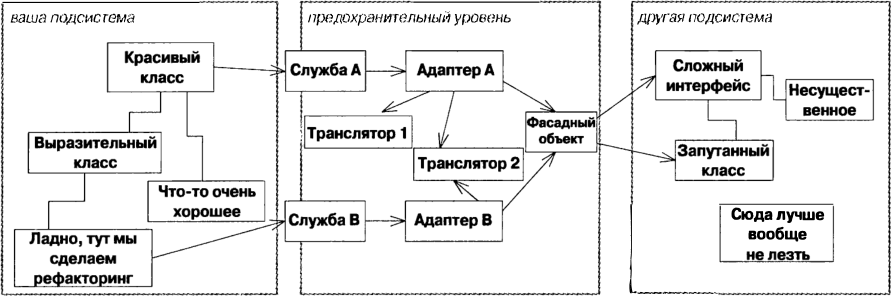
\includegraphics[width=0.9\textwidth]{anticorruptionLayer.png}
\end{center}

\subsubsection{Отдельное существование}

Паттерн <<Отдельное существование>> (Separate Ways) применяется, когда даже <<Предохранительный уровень>> неприменим (например, из-за дороговизны разработки подсистемы преобразования), или вообще в ситуациях, когда преимущества от интеграции меньше затрат на неё. <<Отдельное существование>>, как понятно из паттерна, предполагает отсутствие интеграции вообще --- вы принимаете решения игнорировать существование другого проекта и не пытаться оттуда ничего переиспользовать. 

Хороший жизненный пример применения такого паттерна --- командная работа над дипломом. В некоторых ситуациях какая-либо запланированная интеграция реализаций разных дипломов может быть очень плохой идеей, даже если несколько дипломов пишутся в одном проекте по очень похожим задачам и могут активно переиспользовать функциональность друг друга. В этом случае риски и потенциальный ущерб от их осуществления существенно превышают возможные преимущества от интеграции, даже если сама интеграция и недорога --- кто-то из участников может уйти в академ или просто не осилить, остальным тоже уходить в академ?

\subsubsection{Служба с открытым протоколом}

Паттерн <<Служба с открытым протоколом>> (Open Host Service) --- это что-то вроде <<Заказчик-Поставщик>> со стороны поставщика, у которого уж очень много заказчиков, так что приглашать их всех на planning-сессии и учесть все их пожелания не получится. В этом случае рекомендуется в каком-то смысле вообще не рассматривать <<хотелки>> заказчиков (за исключением требований) и строить модель предметной области самим. После чего предоставить публичный интерфейс, представляющий эту модель, и опубликовать саму модель вместе с интерфейсом (обычно в виде текстовой документации). А заказчикам предлагается самим подстраиваться под опубликованную модель (применяя паттерн <<Конформист>>, или <<Предохранительный уровень>>, если они сильно недовольны).

Пример использования такого подхода --- это большинство публичных REST-сервисов, таких как VK API, Google Drive API и т.д. Публикуются сами сервисы и документация, в которой объясняется, какими сущностями и как эти сервисы манипулируют. При этом обратите внимание, что модель предметной области и единый язык опубликованного сервиса может отличаться от модели предметной области и единого языка, используемого в его реализации. Как правило, <<внешнюю>> модель стараются сделать как можно более простой, тогда как в реализации можно (и часто требуется) разгуляться по полной.

\subsubsection{Общедоступный язык}

Паттерн <<Общедоступный язык>> (Published Language) применяется, когда предметная область достаточно популярна, чтобы в ней появилось очень много <<заказчиков>> и много <<поставщиков>>. Тогда рекомендуется общими усилиями разработать модель предметной области, удовлетворяющую всех поставщиков, стандартизовать её и навязать заказчикам. Эта общая модель предметной области не должна навязывать ничего касательно реализации и должна быть максимально простой, но вместе с тем достаточно выразительной. Для реализации компонентов и сервисов в рамках этой модели могут использоваться свои ограниченные контексты (и не одни), не обязательно совпадающие с опубликованной моделью. Общая модель служит скорее языком и общей средой для общения различных систем в предметной области. 

Примеры применения такого подхода --- это языки программирования (например, компиляторы C++ поставляются несколькими известными производителями, но это более-менее один язык, то же с UML) и отраслевые стандарты --- например, стандарты хранения и передачи медицинских данных, типовые архитектуры авионики или автомобильного бортового программного обеспечения. Стандарты фиксируют общую понятийную базу и терминологию (единый язык) и связь между понятиями (модель предметной области), которым должны следовать все, работающие по стандарту. 

Кстати, стандарт IEEE 1016-2009, упоминавшийся в первой лекции этого курса, --- это как раз пример стандарта с общедоступным языком. Там прямо с использованием UML описывалась предметная область архитектурных видов и предлагался единый язык.

\subsubsection{Сравнение подходов к интеграции}

Взаимосвязь различных  подходов к интеграции ограниченных контекстов описывает рисунок из книги Эванса: 

\begin{center}
    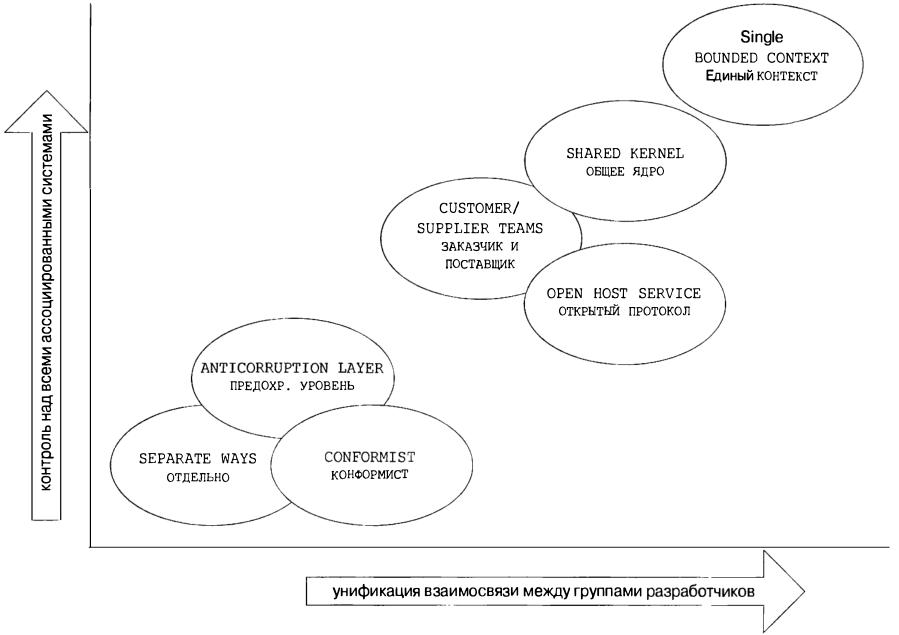
\includegraphics[width=0.8\textwidth]{integrationPatterns.png}
\end{center}

В правом верхнем углу находится полная интеграция --- когда команды работают в едином ограниченном контексте. Это требует максимальной взаимосвязи между группами разработчиков (на самом деле, по факту это должна быть одна команда) и максимального контроля над кодом (на самом деле, кодовая база должна быть полностью подвластна команде). Чуть слабее требования у паттерна <<Общее ядро>>. Дальше стоят <<Заказчик-Поставщик>> и <<Открытый протокол>> --- при этом <<Заказчик-Поставщик>> позволяет влиять на компонент, от которого мы зависим, <<Открытый протокол>> в меньшей степени, зато требует существенно больше документации (поэтому требуется больше коммуникации, хоть и односторонней).

В левом нижнем углу находятся паттерны, применяемые, кода всё плохо. <<Предохранительный уровень>> --- кода мы хотим писать какой-то код, чтобы защитить своё миропонимание от навязанного третьесторонним компонентом (так что требует много кода), <<Конформист>> --- когда не хотим, но тогда нам надо болше разбираться в миропонимании компонента (оттого больше коммуникации, даже если она заключается в чтении документации и кода). И наконец, <<Отдельное существование>> не требует ни коммуникации, ни какого-либо контроля, но и интеграции никакой не даёт.

\subsection{Пример: унификация слона}

Небольшой метафорический, но на самом деле очень жизненный пример применения паттернов интеграции из книги Эванса основывается на стихотворении <<Слепцы и слон>> Дж. г. Сакса (1816--1887):

\begin{verse}
    Шесть седовласых мудрецов \\
    Сошлись из разных стран. \\
    К несчастью, каждый был незряч, \\
    Зато умом блистал. \\
    Они исследовать слона \\
    Явились в Индостан. \\!

    Один погладил бок слона. \\
    Довольный тем сполна, \\
    Сказал он: ``Истина теперь \\
    Как божий день видна: \\
    Предмет, что мы зовем слоном, ­\\
    Отвесная стена!'' \\!

    А третий хобот в руки взял \\
    И закричал: ``Друзья! \\
    Гораздо проще наш вопрос, \\
    Уверен в этом я! \\
    Сей слон --- живое существо, \\
    А именно змея!'' \\!

    Мудрец четвертый обхватил \\
    Одну из ног слона \\
    И важно молвил: ``Это ствол, \\
    Картина мне ясна! \\
    Слон --- дерево, что зацветет, \\
    Когда придет весна!'' \\!

    Тем временем шестой из них \\
    Добрался до хвоста. \\
    И рассмеялся от того, \\
    Как истина проста. \\
    ``Ваш слон --- веревка. Если ж нет \\
    Зашейте мне уста!'' \\!

    А как известно, мудрецам \\
    Присущ упрямый нрав. \\
    Спор развязав, они дошли \\
    Едва ль не до расправ. \\
    Но правды ни один не знал, \\
    Хотя был в чем-то прав.
\end{verse}

Шесть мудрецов --- это шесть команд разработчиков, работающих над одним проектом в шести ограниченных контекстах. Посмотрим, как они могли бы постепенно интегрировать свои контексты, улучшая в процессе интеграции качество модели и своё понимание предметной области.

Первый вариант интеграции --- отсутствие интеграции как таковой, почти как в оригинальном стихотворении. Это соответствует паттерну <<Раздельное существование>>, когда каждый мудрец имеет свою точку зрения, придерживается её и не лезет в другие ограниченные контексты. Системы не могут интегрироваться друг с другом и их модели предметной области радикально различны:

\begin{center}
    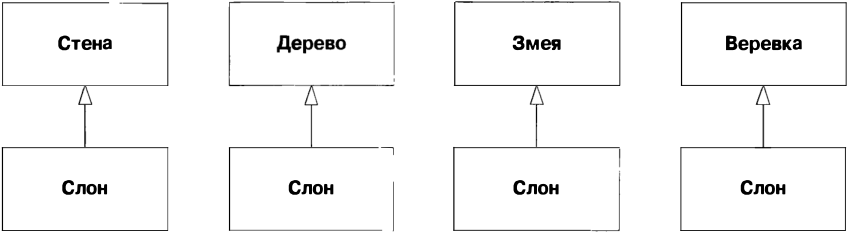
\includegraphics[width=0.8\textwidth]{elephantSeparateWays.png}
\end{center}

Некоторая минимальная интеграция могла бы быть получена с помощью паттерна <<Предохранительный уровень>>. Каждый мудрец всё ещё считает, что остальные понимают предметную область неправильно, но они могут договориться о схеме трансляции между понятиями: 

\begin{center}
    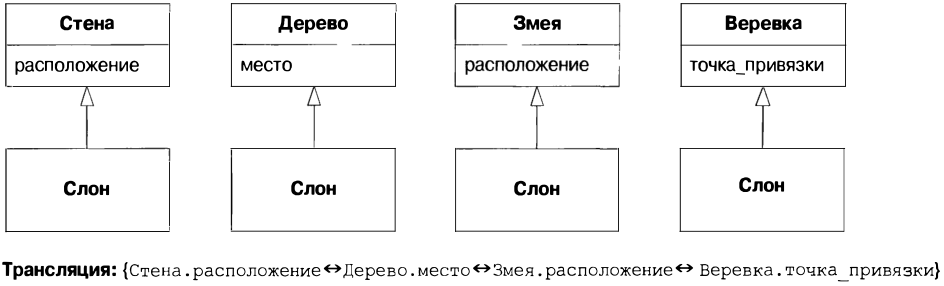
\includegraphics[width=0.9\textwidth]{elephantAnticorruptionLayer.png}
\end{center}

Теперь у всех моделей есть некоторые свойства, которые по оговоренным заранее правилам могут преобразовываться друг в друга. Не всегда это преобразование тривиально, не всегда сохраняет все данные, не всегда имеет смысл в рамках <<настоящей>> предметной области, но всё-таки позволяет системам работать совместно. Например, мудрец, считающий слона стеной, может определить расположение стены, которое может быть так или иначе транслировано в точку привязки верёвки для мудреца, который считает слона верёвкой. 

Стоит отметить, что и в реальной жизни <<настоящая>> предметная область далеко не очевидна, особенно в начале разработки, особенно если разработка ведётся в сфере, далёкой от жизненного опыта разработчиков (например, информационная система для автомобильного завода или даже информационная система поддержки учебных практик СПбГУ). Если несколько команд работают над одной областью и анализируют её независимо (например потому, что относятся к разным организациям и просто не знают о существовании друг друга), они будут действовать в точности как слепые мудрецы и проблемы на первых этапах интеграции, если она начнётся, практически неизбежны.

Следующий этап --- это выделение общего ядра. В оригинальном стихотворении мудрецы просто разругались, в мире программирования всё же более типична ситуация, когда команды продолжают работать вместе и находят общие фрагменты своих моделей, что становится основой интеграции:

\begin{center}
    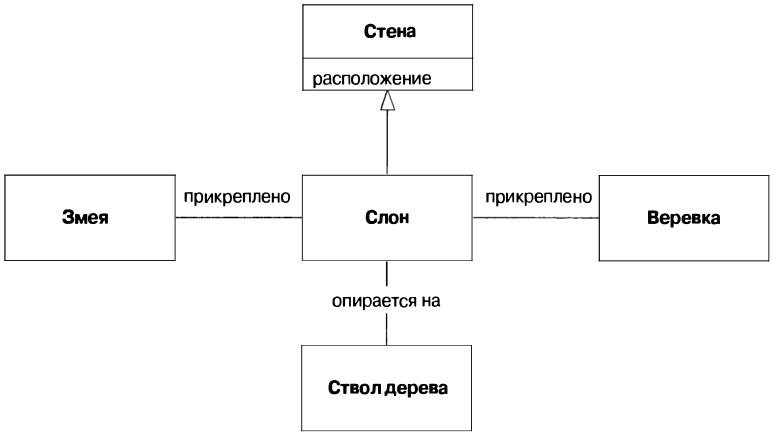
\includegraphics[width=0.8\textwidth]{elephantSharedKernel.png}
\end{center}

Тут мудрецы уже поняли, что говорят по сути об одном, но каждый всё ещё наделяет слона своими своствами, специфичными для его точки зрения. Тем не менее, они уже могут рассуждать в терминах общей и понимаемой ими однозначно сущности <<Слон>>. При этом одному из мудрецов повезло и его класс <<Стена>> был принят как предок для класса <<Слон>>, так что мудрецы согласились, что у слона есть расположение. Но это не значит, что класс <<Стена>> сам принадлежит смысловому ядру: всё, что от него можно унаследовать, то есть состояние, поведение и инварианты --- да, безусловно, но вряд ли мудрецы бы согласились включить в единый язык общего ядра тот факт, что слон является стеной. А в DDD общий язык важнее технических соображений.

Ну и последний этап интеграции --- когда мудрецы достигают полного согласия и формируют единый ограниченный контекст:

\begin{center}
    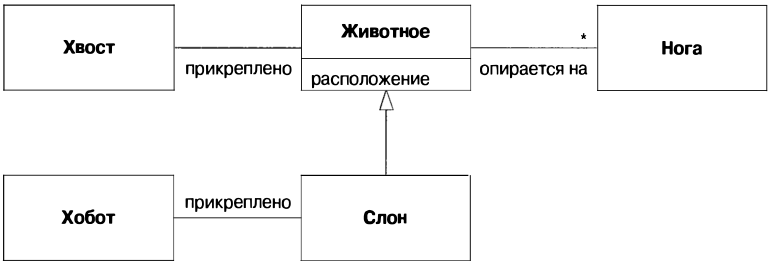
\includegraphics[width=0.8\textwidth]{elephantSingleBoundedContext.png}
\end{center}

Таким образом, команды разработчиков, в отличие от мудрецов, с помощью постепенной интеграции всё-таки смогли установить истину и собрать из фрагментов единую модель предметной области, в которой могут работать, пока снова не разругаются.

\section{Смысловое ядро}

Ключевой момент предметно-ориентированного проектирования больших систем --- это выделение их самой содержательной части, вынесение из неё всего, непосредственно к ней не относящегося, и акуратный её дизайн. Эта содержательная часть предметной области называется \textit{смысловое ядро} (Core Domain) --- это то, что, собственно, делает систему ценной. То, за что, собственно, заказчики платят деньги. Например, в любой информационной системе есть библиотека для работы с базой данных, скорее всего, какая-то сетевая часть, скорее всего, какой-то UI. Но полезна информационная система только тогда, когда правильно моделирует данные и бизнес-процессы заказчика. Или компьютерная игра --- вы можете потратить кучу времени на реализацию сохранения-загрузки, но купят игру либо из-за интересной игровой механики, либо из-за хорошего дизайна, либо ещё из-за чего-то, с сохранением и загрузкой не связанного. Сохранение и загрузка тоже важны, и без них игру не купят, но это не главное.

Только смысловое ядро фактически составляет know-how, то, что выделяет ваш продукт на фоне конкурентов и то, что представляет настоящую ценность, всё остальное в принципе можно смело выложить в open source (а лучше взять из open source, потому что наверняка уже десять раз реализовано). Пожтому смысловое ядро должно быть самой проработанной частью системы. Причём, ирония состоит в том, что опытные программисты не любят заниматься смысловым ядром, потому что оно требует глубокого погружения в предметную область. Гораздо приятнее заниматься базами данных или UI и написать потом в резюме длинный список технологий, которыми ты мастерски владеешь, чем написать в резюме, что ты прекрасно разбираешься в работе логистических компаний (и тогда тебя трудоустроят те две-три компании в мире, которые делают свой бизнес на автоматизации в сфере логистики) или ты эксперт в размножении тушканчиков и умеешь строить отличные предметно-ориентированные модели.

С таким мировоззрением надо бороться. На самом деле, работать на резюме в плане изучения стеков технологий может быть полезно, пока вы junior developer, но ближе к позиции senior уже стратегически невыгодно. Богатый технический бэкграунд к этому моменту постепенно обесценится из-за естественной смены модных технологий, и с вами на рынке труда будут конкурировать junior-ы, которые на новых технологиях выросли, и поэтому знают их лучше вашего. Да и вряд ли вы к тому времени будете хотеть juniorскую зарплату. А вот специализация в некоторой предметной области junior-ам недоступна, поскольку требует массы времени и усилий уже после базового образования, и, хоть и сужает возможности трудоустройства, делает вас ценным специалистом, которого самого приглашают на работу, причём на очень высокую зарплату (потому что такие специалисты редки). В мире миллионы Java-программистов, но программист, шарящий в размножении тушканчиков, возможно, один, и если кому-то он понадобится, за него отдадут любые деньги. Например, молодых выпускников матмеха, успевших специализироваться в компьютерной криминалистике, несмотря на небольшое количество работодателей в этой сфере, перекупали друг у друга у меня на глазах.

\subsection{Дистилляция}

Смысловое ядро, поскольку оно самая важная часть системы, должно быть как можно меньше (чтобы с ним легче было работать) и чётко отделённым от остальных компонентов системы. Процесс выделения смыслового ядра Эванс называет \textit{дистилляцией} и приводит несколько дельных советов про то, как это делать.

Первый приём, позволяющий выделить смысловое ядро --- это Domain Vision Statement. Domain Vision Statement --- это короткий документ (примерно на одну страницу), описывающий смысловое ядро и его полезность. Обычно его имеет смысл делать в самом начале проекта, вместе с описанием проекта вообще. В реальной жизни ни разу такого не видел, однако видел ``устав проекта'', где, в частности, и описывается то, что должно быть в Domain Vision Statement. Тем не менее, охотно поверю в полезность такого документа. Смысл тут в том, чтобы документ был коротким и ёмким, не надо описывать архитектуру ядра, надо описать, что оно умеет и зачем оно.

Выделенное ядро (Highlighted Core) --- это способ уже на готовой модели обозначить смысловое ядро. Бывает двух видов. Первый --- \textit{дистилляционный документ} --- это 3-7 страниц текста про то, что составляет смысловое ядро и как его элементы взаимодействуют друг с другом. По сути, развёрнутый Domain Vision Statement, с архитектурой смыслового ядра, как правило, часть архитектурной документации. Второй --- Flagged Core --- это когда элементы ядра выделены на существующей модели, например, специальным стереотипом или даже просто цветом. Дёшево и вместе с тем достаточно эффективно.

Далее выполняется собственно дистилляция, то есть избавление кода смыслового ядра от всего лишнего. Делается это вынесением неспецифичной для приложения функциональности в отдельные модули. СОбственно видов неспецифичной функцональности в DDD выделяют два:

\begin{itemize}
    \item Неспециализированные подобласти (Generic Subdomains) --- куски кода, важные для предметной области, но неспецифичные для конкретной системы;
    \item Связный механизм (Cohesive Mechanism) --- куски кода, неспецифичные для предметной области вообще. Это могут быть разные технические вещи, например, раота с графами. Иногда оказывается, что хитрая структура самописных классов --- это не более чем замаскированный граф, и тогда стоит просто изменить архитектуру так, чтобы можно было переиспользовать одну из готовых библиотек. Связные механизмы принципиально отличаются от неспециализированных подобластей тем, что они уж точно тысячу раз реализованы и имеет смысл выбрать готовый компонент. С несециализированными подобластями тоже может повезти, а может, их реализации можно взять из других проектов компании, но с большой вероятностью их придётся писать самим (хоть они и не смысловое ядро системы).
\end{itemize}

\subsection{Пример, грузоперевозки}

Рассмотрим дистилляцию модели на примере логистической системы с прошлой пары. Напомним, что мы проектировали систему, позволявшую заказать доставку груза (Cargo), по маршруту (Itinerary), удовлетворяющему спецификации (Route Specification) и состоящему из шагов (Handling Step) и перевозок (Leg):

\begin{center}
    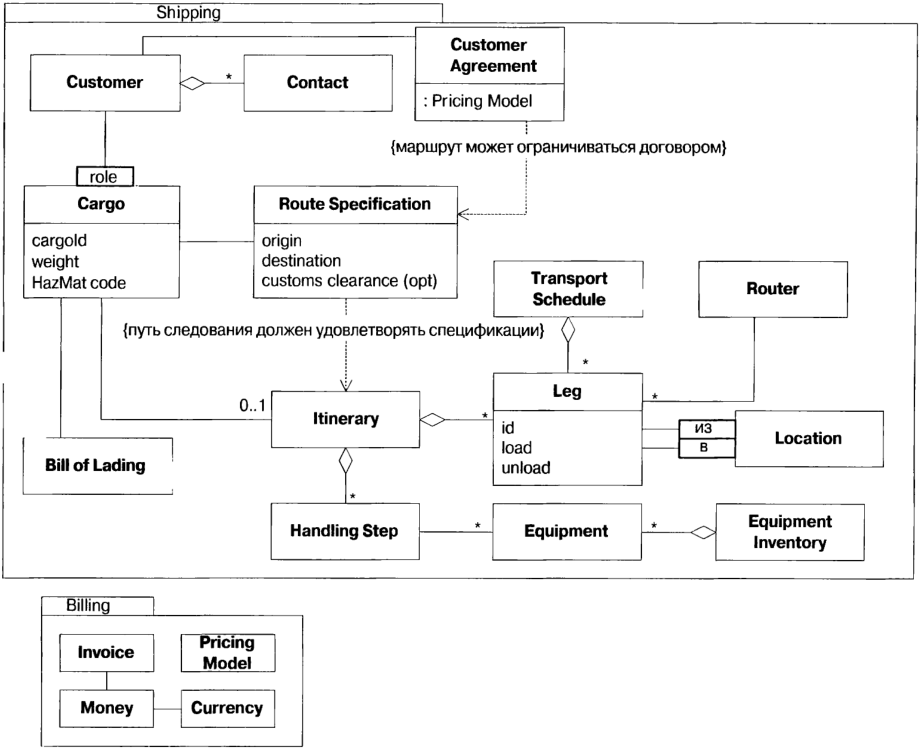
\includegraphics[width=0.9\textwidth]{shippingRaw.png}
\end{center}

Посмотрев на эту систему внимательно, мы понимаем, что тут есть классы, относящиеся собственно к доставке груза, к прокладке маршрута, к работе с клиентом и всякие явно вспомогательные классы. Поскольку основной бизнес нашей компании --- это организация перевозок, смысловым ядром для нашей системы будут классы, которые непосредственно занимаются доставкой. Это Cargo (груз, мы его, собственно, доставляем), RouteSpecification (это то, откуда, куда и как мы везём груз, критическая для нашего бизнеса часть модели), Itinerary, Handling Step (это наша основная работа на самом деле), BillOfLading (ключевой для нашей работы документ) и CustomerAgreement (потому что всё это на самом деле нужно для выполнения обязательств по договору).

А вот сам Customer и его контакты к смысловому ядру не относятся --- это умеют любые CRM-системы в разы лучше нас. Перевозка, расписание транспорта, даже прокладка маршрута --- это не ядро нашего бизнеса, хотя и, безусловно, важно. Большая часть этого --- это вообще задачи транспортных компаний, и соответствующие классы мы используем просто как данные. Прокладка маршрута и составление расписания интереснее, но есть специальные библиотеки, которые этим занимаются и умеют делать хорошо --- опять-таки, это важная часть нашего бизнеса, но не то, за что нас будут любить клиенты, не то, что мы хотим уметь делать лучше всех в мире.

В результате рефакторинга может получиться вот такая модель (<<flagged core>>):

\begin{center}
    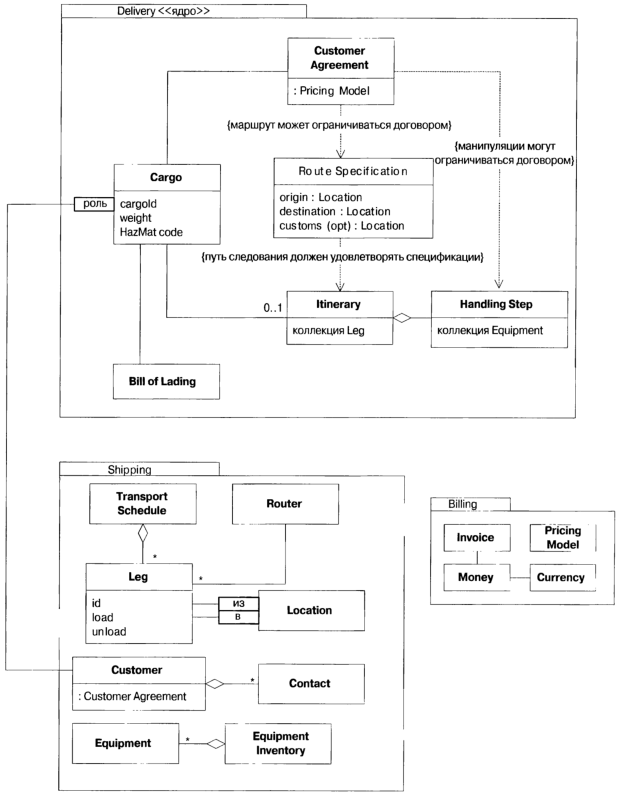
\includegraphics[width=0.9\textwidth]{shippingDistilled.png}
\end{center}

Как видим, сложность смыслового ядра уменьшилась вдвое.

Однако и на этом останавливаться ещё рано --- модуль Shipping нарушает принцип единственности ответственности, так что его можно разбить на два: Customer и Logistics. В Customer пойдут классы, ответственные за работу с клиентом (Customer, Contact), в Logistics --- всё, что связано с перевозками. При этом мы можем заметить, что в можуле Billing есть классы Invoice и PricingModel, которые специфичны для нашего бизнеса, и Money с Currency, которые нет. Давайте вынесем Invoice и PricingModel в модуль Customer (это оправданно потому что модель ценообразования и выставление счетов явно относятся к клиенту и вполне могут от него сильно зависеть), и тогда можно Money с Currency оставить в одном модуле и сделать его неспециализированной подобластью. Тогда получится вот такое:

\begin{center}
    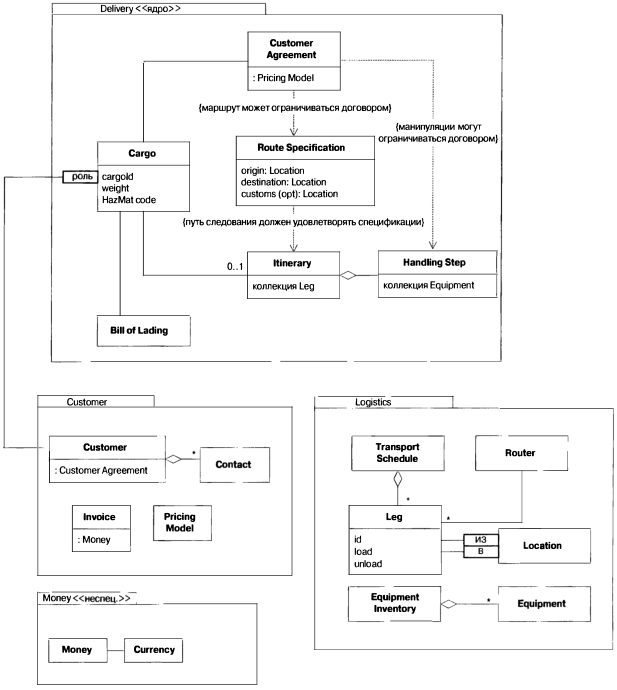
\includegraphics[width=0.9\textwidth]{shippingRepacked.png}
\end{center}

\subsection{Абстрактное ядро}

Иногда даже после этих ухищрений смысловое ядро остаётся всё ещё слишком большим, чтобы его можно было адекватно сопровождать. Тогда можно применить приём <<Абстрактное ядро>> --- когда смысловое ядро состоит только из абстрактных классов/интерфейсов, которые потом реализуются отдельными модулями. Радикально сложность модели это всё равно не уменьшит (но так и должно быть, это <<essential complexity>>), но хотя бы позволит избавиться от ненужных подробностей реализации. Схема такая:

\begin{center}
    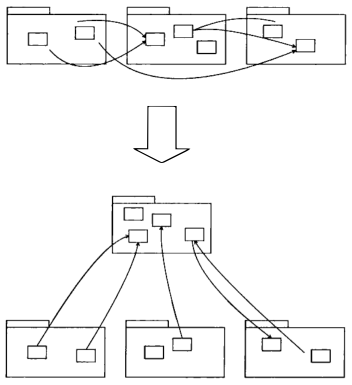
\includegraphics[width=0.5\textwidth]{abstractCore.png}
\end{center}

\section{Крупномасштабная структура}

Крупномасштабная структура --- это самая <<архитектурная>> часть архитектуры, набор основных правил, которым следует вся система или группа систем. Например, может быть задекларировано, что система в целом имеет уровневую архитектуру, и уровни такие-то и такие-то. Тогда как реализация самих уровней может выполняться в совершенно разных архитектурных стилях. Более того, просто задекларировать, что система имеет уровневую архитектуру --- это уже зафиксировать её крупномасштабную структуру, хоть и слишком общую, чтобы быть реально полезной. Вообще, крупномасштабная структура системы --- это чаще всего уточнённый под конкретную систему архитектурный стиль плюс набор специфичных для системы ограничений (например, перечисление основных компонентов и их ответственностей, правила, по которым в систему можно добавлять новые компоненты).

Крупномасштабная структура не фиксируется раз и навсегда, как бы ни был велик соблазн это сделать. По мере роста понимания предметной области в процессе \textit{переработки знаний} и по мере получения обратной связи о том, насколько удобна выбранная архитектура в коде крупномасштабная архитектура вполне может меняться и эволюционировать (естественно, совместно с моделью и с кодом). Кроме того, не следует делать её слишком жёсткой и пытаться всё предусмотреть (раз она может эволюционировать, её всегда можно будет потом поправить). Тем более не следует использовать административный ресурс, чтобы принуждать разработчиков ей следовать. Организация команды <<Архитектор в башне из слоновой кости>>, когда архитектор разрабатывает архитектуру, но сам код не пишет и не прислушивается к обратной связи от программистов, зарекомендовала себя на практике очень плохо, кроме того, в предметно-ориентированном проектировании её особенно не любят (поскольку она ещё и осложняет ту самую переработку знаний).

Небольшие проекты вполне могут жить без явно задокументированной крупномасштабной структуры --- если у вас всего пять классов, то их взаимоотношения будут вполне достаточны в качестве архитектуры. Более того, пытаться <<архитектурить>> небольшой скрипт или утилиту может быть саботажем сроков и стоимости проекта, особенно если реализация архитектурных мечтаний требует написания большого количества кода. 

Но надо принимать во внимание, что все большие проекты начинались как небольшие, и если о крупномасштабной структуре не подумать, в какой-то момент возникнет хаос. Причём, совершенно не требуется сразу, как только вы написали первый маленький классик, продумывать плагинные системы, миграции, шины интеграции и т.п., ведь крупномасштабная структура может эволюционировать. Сначала стоит зафиксировать хоть какую-то, затем постепенно её корректировать и уточнять.

Ещё стоит отметить, что крупномасштабная структура --- это не огромный архитектурный документ с изобилием UML-диаграмм и ссылок на стандарты (хотя если такой есть, то это не плохо), это вполне может быть устная традиция, передаваемая от разработчика к разработчику. Вообще, самый полезный носитель крупномасштабной структуры по DDD --- это \textit{единый язык} и его термины. Если в ходе общения сам собой выкристаллизовался слой А, слой Б и появился набор правил в духе <<нет-нет, мы так не делаем>> --- это уже вполне нормально в качестве крупномасштабной структуры, особенно если все понимают её однозначно (а должны, это ведь единый язык).

В этом плане очень полезна \textit{метафора системы} --- некая аналогия, определяющая, как в целом понимать систему. Разные метафоры используются в программировании повсеместно, из-за незримости ПО и желания всё-таки его как-то представлять. Например, метафора рабочего стола для пользовательских интерфейсов, файервола в сетевой безопасности и т.д., даже деревья в программировании называются деревьями, потому что похожи на... деревья (а могли бы --- связными ациклическими графами). Однако метафору не всегда легко подобрать, и она не всегда оказывается удачной. 

Особо опасна метафора тем, что тащит за собой лишний смысл из реальной жизни. Например, файервол ассоциируется с противопожарной перегородкой, разделяющей разные части сети, и если понимать её слишком буквально, можно забыть, что файервол должен контролировать и локальный трафик. Или тот же рабочий стол --- в ральной жизни не бывает рабочих столов, бесконечных во все стороны, поэтому и рабочие столы на компьютере ограничены (хотя, наверное, было бы удобно иметь скроллящийся как карта в реал-тайм стратегиях рабочий стол, особенно управляемый движением головы, взглядом или вообще VR). Тем не менее, хорошая метафора, особенно из предметной области проекта, может сильно помочь.

Наиболее типичная крупномасштабная структура --- это уроневая. Уровневый архитектурный стиль мы неоднократно уже обсуждали, но есть ещё одно важное соображение, касающееся использования уровней как именно крупномасштабной структуры --- нельзя чисто механически делить систему на уровни топологической сортировкой графа зависимостей компонентов. Например,

\begin{center}
    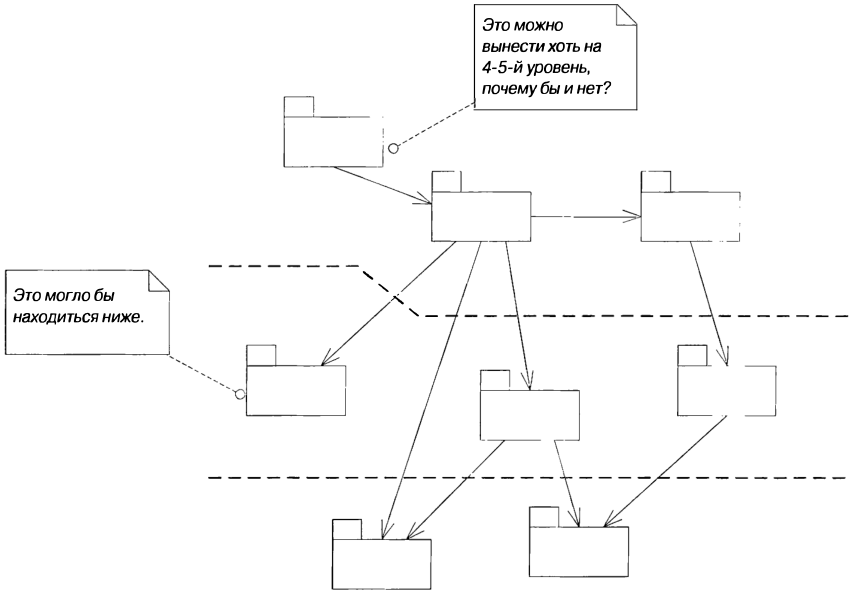
\includegraphics[width=0.7\textwidth]{meaninglessLayers.png}
\end{center}

Разбиение по уровням, как и любое разбиение в архитектуре вообще, должно сообщать дополнительную информацию об идее реализации системы, выражать мысль архитектора и объяснять происходящее. Причём, объяснять --- на самом деле, самое важное: качество архитектуры, как научной теории в представлении философов науки 20-го века, определяется её объясняющей способностью. Не важно, что архитектура позволяет быстро или эффективно что-то реализовать, она всё равно плоха, если не объясняет происходящего.

Кстати, поэтому результаты автоматической генерации диаграмм по коду --- не архитектура ни разу.

Чтобы избежать бессмысленного разбиения на уровни, надо каждому уровню придать какое-то значение из предметной области и ограничения, с ним связанные. Рассмотрим эту мыфсль подробнее на примере.

\subsection{Пример, перевозка грузов}

Пример рефакторинга системы к осмысленной уровневой крупномасштабной структуре, как обычно, рассмотрим на системе про грузоперевозки. Напомним, что у нас есть груз, который надо доставить в соответствии со спецификацией маршрута, для чего мы с помощью класса Router генерим расписание (Itinerary) перевозки:

\begin{center}
    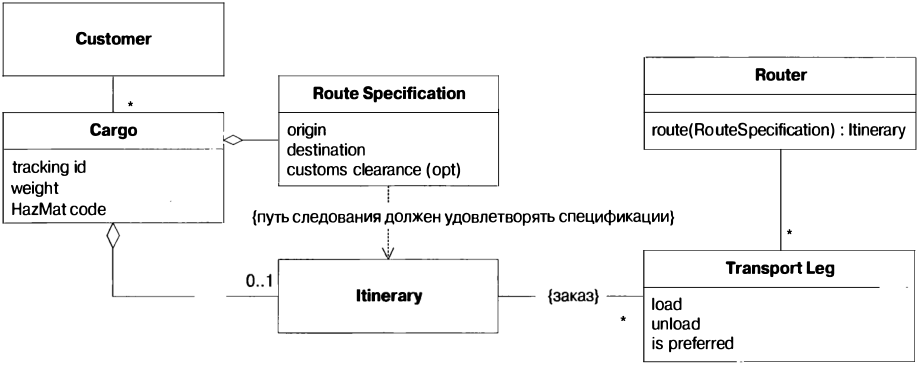
\includegraphics[width=0.9\textwidth]{cargoNonLayered.png}
\end{center}

Система небольшая, так что кажется, что искусственно бить её на уровни нет смысла. Но мы понимаем, что система будет расти, и хотим придумать какое-то простое правило, которое бы объясняло, куда добавлять какие классы и как они должны вписываться в уже существующую систему, чтобы не получился огромный клубок из взаимосвязанных классов. Для начала рассмотрим поближе, как в текущей архитектуре работает типичный запрос, заказ перевозки:

\begin{center}
    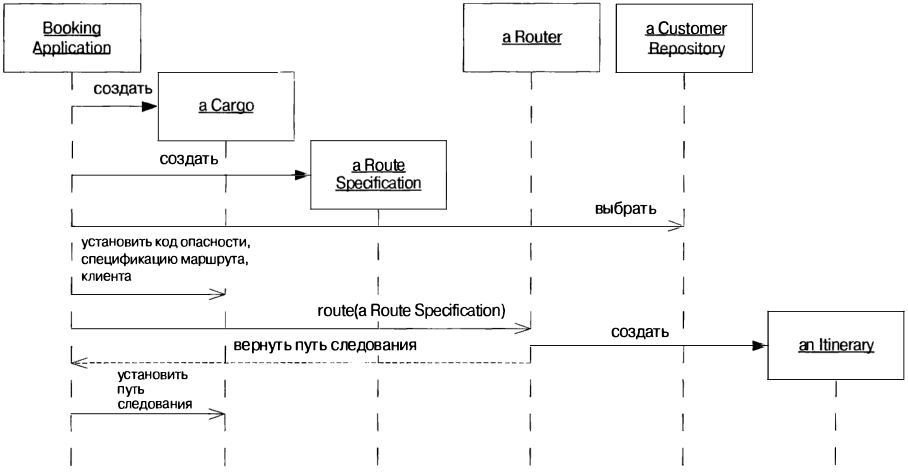
\includegraphics[width=0.9\textwidth]{cargoNonLayeredSequence.png}
\end{center}

Приложение, бронирующее перевозку, сначала создаёт Груз, коорый надо перевести, затем Спецификацию маршрута (где Груз забрать и куда и когда его надо доставить). Далее оно выбирает из репозитория объект Клиент, который использует для инициализации Груза, и отдаёт то, что получилось, в Маршрутизатор, который создаёт и возвращает Расписание перевозки. Расписание устанавливается Грузу, и после этого он готов к поездке.

Можно заметить, что планирование маршрута использует клиента просто как данные, и строит расписание, которое на самом деле состоит из Перевозок, которые реализуются компаниями-перевозчиками (в отличие от нас, владеющими реальными средствами перевозки), так что для наз Перевозки --- это тоже просто данные. Возникает идея это явно отразить в архитектуре, разделив её на два уровня --- Операционный и Ресурсный. Ресурсный уровень представляет то, что обеспечивает наши возможности (перевозчики, и, как ни странно, клиент --- он нам деньги платит, заказывает перевозки, и мы им не управляем никак). Операционный уровень --- это то, как мы пользуемся нашими возможностями, тут будут классы, отвечающие за оперативное управление процессами и планирование. Очевидно, Customer и Transport Leg пойдут на ресурсный уровень, остальное --- на операционный.

Ещё мы хотим топологическое ограничение --- объекты уровня ниже не могут знать про объекты уровня выше (иначе толку от разделения на уровни никакого). Однако в нашей исходной модели Customer знает про Cargo (ну а что, он же должен знать про заказанные перевозки), и про Transport Leg не указаны направленности ассоциаций. Во втором случае проблем нет, перевозчик ничего не должен знать про Маршрутизатор и Расписание даже по логике вещей, а вот с Customer и Cargo реально потребуется рефакторинг. Но мы уже умеем так делать с прошлой лекции: используем паттерн <<Репозиторий>>: 

\begin{center}
    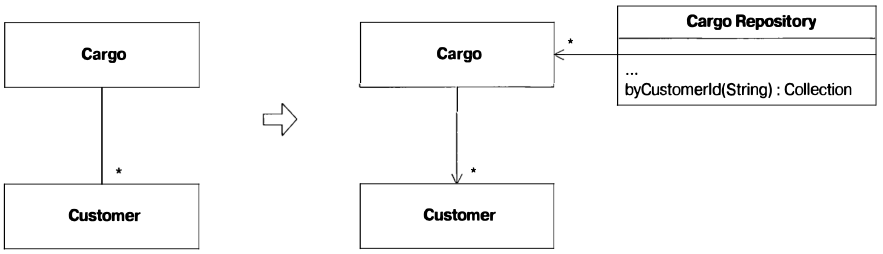
\includegraphics[width=0.9\textwidth]{cargoTwoLayersRefactoring.png}
\end{center}

Теперь Груз знает про Клиента, но Клиент не знает прои груз, однако может при желании получить его из репозитория грузов. Все репозитории глобально доступны, так что в уровневую структуру в любом случае не вписываются, они как бы живут параллельно. Топологии системы это не ломает, потму что репозитории ссылки не хранят, да и на них никто не хранит ссылок. После рефакторинга получилось как-то так:

\begin{center}
    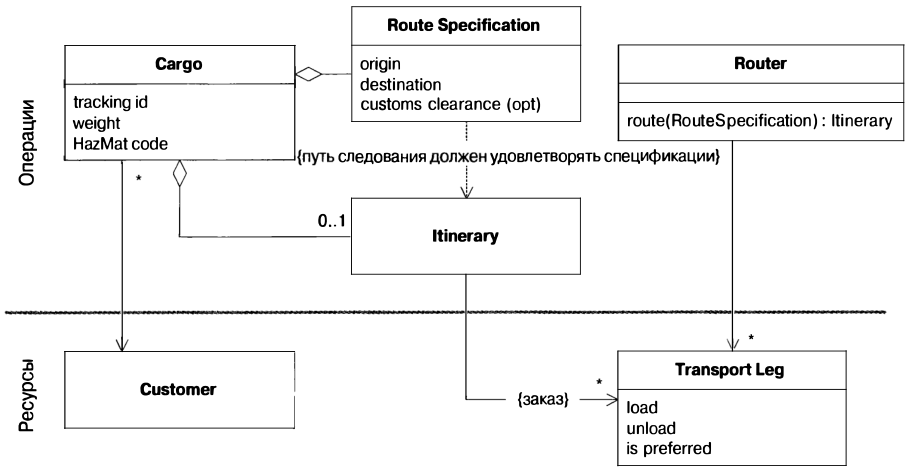
\includegraphics[width=0.9\textwidth]{cargoTwoLayers.png}
\end{center}

Стало лучше. Однако вспомним, как мы определили операционный уровень: <<это то, как мы пользуемся нашими возможностями, тут будут классы, отвечающие за оперативное управление процессами и планирование>>. <<управление процессами и планирование>> звучит так, будто на самом деле мы хотим два уровня, <<управление процессами>> и <<планирование>> --- уровень Поддержки решений будет работать только иногда и строить план, который должен претворять в жизнь Операционный уровень. Очевидно, на уровень Поддержки решений отправляется класс Router, который по данной 
Спецификации маршрута должен построить нам Расписание. Спецификацию маршрута и Расписание можно оставить на операционном уровне, потому что про них должен знать Груз, чтобы исполнять нужные перевозки (на самом деле, насчёт Спецификации маршрута спорно, но при заказе мы указываем груз и Спецификацию маршрута, и они всегда ходят вместе в нашей системе, так что давайте пока так --- это типа маршрутного листа, который едет вместе с грузом, ему тогда самое место на операционном уровне).

Есть, однако, проблема, проистекающая из предметной области. У Transport Leg есть поле <<is preferred>>, которое true, если перевозку мы выполняем на нашем же транспортном средстве или силами компании-партнёра. Такие перевозки для нас предпочтительны, потому что зачем нам делиться прибылью с чужими людьми? Однако это явно поле, нужное только на этапе планирования, и нужное только для Маршрутизатора при построении Расписания. Поэтому давайте его поднимем на уровень Поддержки решений, заведя отдельный класс Route Bias Policy, который бы помнил, какие из Перевозок нам больше нравятся. На самом деле, это позволит нам потом реализовать более мощные механизмы маршрутизации, чем даже были задуманы изначально (например, Route Bias Policy может при планировании маршрутов давать меньший вес Перевозкам вокруг Сомали или следить за новостями и не отправлять груз самолётом над зоной активного военного конфликта). Получилось что-то такое:

\begin{center}
    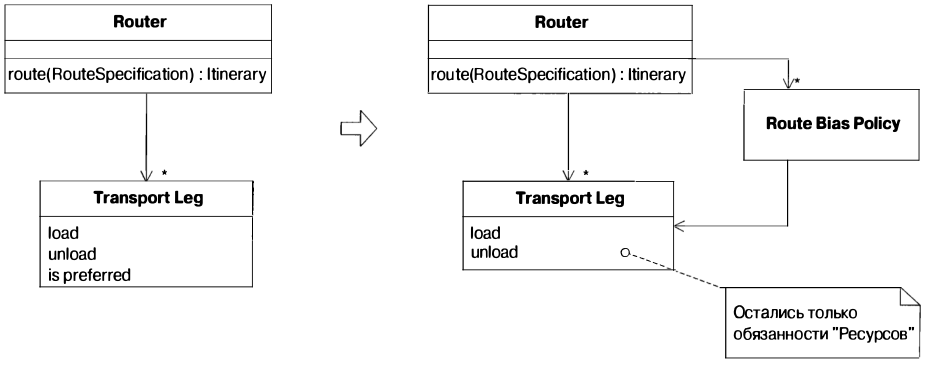
\includegraphics[width=0.9\textwidth]{cargoThirdLayerRefactoring.png}
\end{center}

Ну и итоговая архитектура уже с тремя уровнями:

\begin{center}
    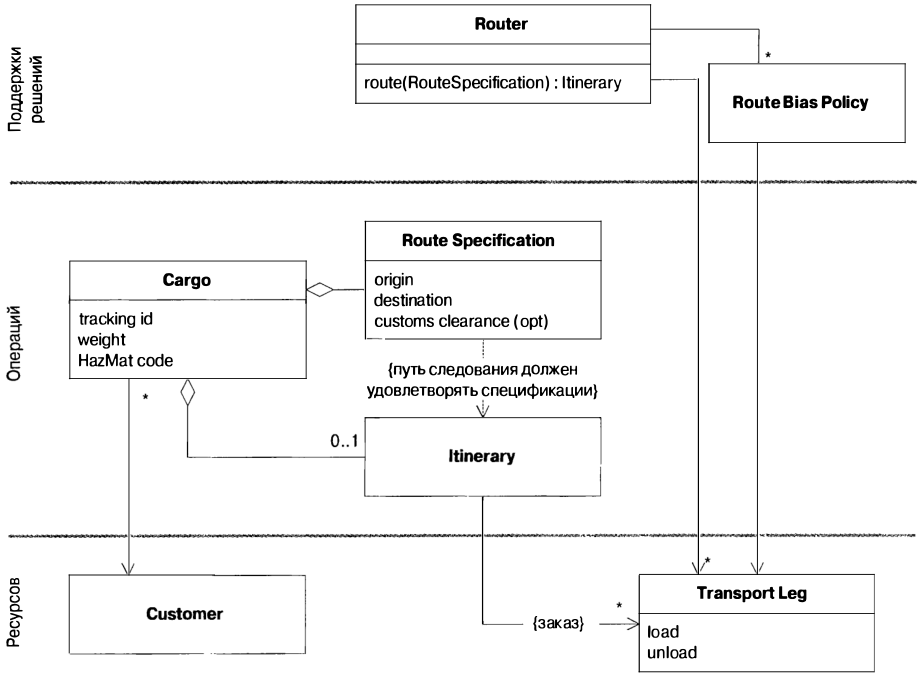
\includegraphics[width=0.8\textwidth]{cargoThreeLayers.png}
\end{center}

Стало ещё лучше, каждый уровень достаточно небольшой, есть чёткое понимание (ну, более-менее чёткое), на каком уровне что должно находиться, есть строгие топологические ограничения насчёт направленности ассоциаций.

И тут внезапно появляется новое требование --- работа с опасными грузами. Их нельзя ввозить в определённые локации (было бы плохой идеей везти радиоактивные отходы через крупный город) и нельзя везти определёнными перевозчиками (попытки доставить Чужих на Землю для изучения, заразив команду корабля или колонистов, постоянно оканчивались провалом). Для поддержки таких дел Грузу добавляется поле <<HazMat code>>, которое, хоть и нужно только на этапе составления Расписания, является неотъемлемым свойством груза, и выносить его в отдельную политику идеологически не очень хорошее решение. Поэтому первое решение, что пришло нам в голову --- это сделать сервис, который бы брал груз и Спецификацию маршрута, и дополнял бы её запретами для конкретного кода опасности:

\begin{center}
    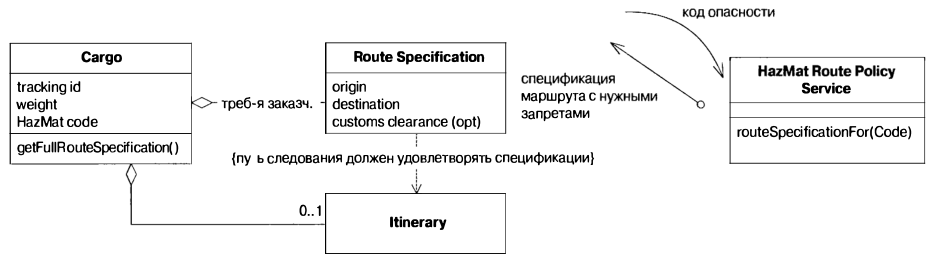
\includegraphics[width=0.95\textwidth]{cargoHazMatWrong.png}
\end{center}

Тогда наша система работала бы так:

\begin{center}
    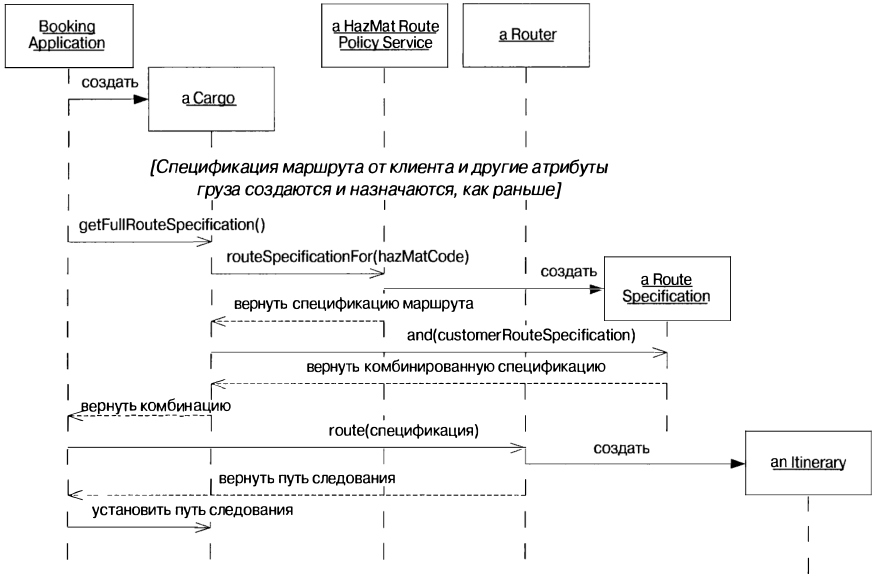
\includegraphics[width=0.85\textwidth]{cargoHazMatWrongSequence.png}
\end{center}

Приложение, в котором Клиент заказывает доставку, как обычно создавало бы груз и Спецификацию маршрута, после чего вызывало бы у Груза получение обновлёной спецификации, для чего Груз запрашивает спецификацию ограничений для своего кода опасности и мерджит её (с помощью метода and) с обычной Спецификацией маршрута, которую нам заказал Клиент (паттерн <<Спецификация>> с композитной спецификацией таки).Ну а дальше Маршрутизатор по данной комбинированной Спецификации маршрута составляет Расписание, которое и назначается Грузу.

Всё хорошо, но нарушает наше ограничение --- политика работы с опасными грузами относится к уровню Поддержки решений, но её вызывает Груз, что заставляет либо перенести её на уровень ниже (что против идеологического разделения на уровни), либо позволить Грузу делать запрос к классу уровня выше (что против топологических ограничений, и тут даже трюк с репозиторием не поможет, поскольку Грузу реально требуется что-то содержательное делать с этим классом). Поэтому предложенная нами архитектура не подойдёт, но еёл егко исправить: давайте не Груз будет получать для себя Спецификацию маршрута, а сам Маршрутизатор (и когда нас посещает эта идея, мы удивляемся, как нам вообще пришла в голову предыдущая архитектура, ведь такое решение очевидно лучше даже без всяких опасных грузов --- \textit{переработка знаний} во всей красе). Вот что получается:

\begin{center}
    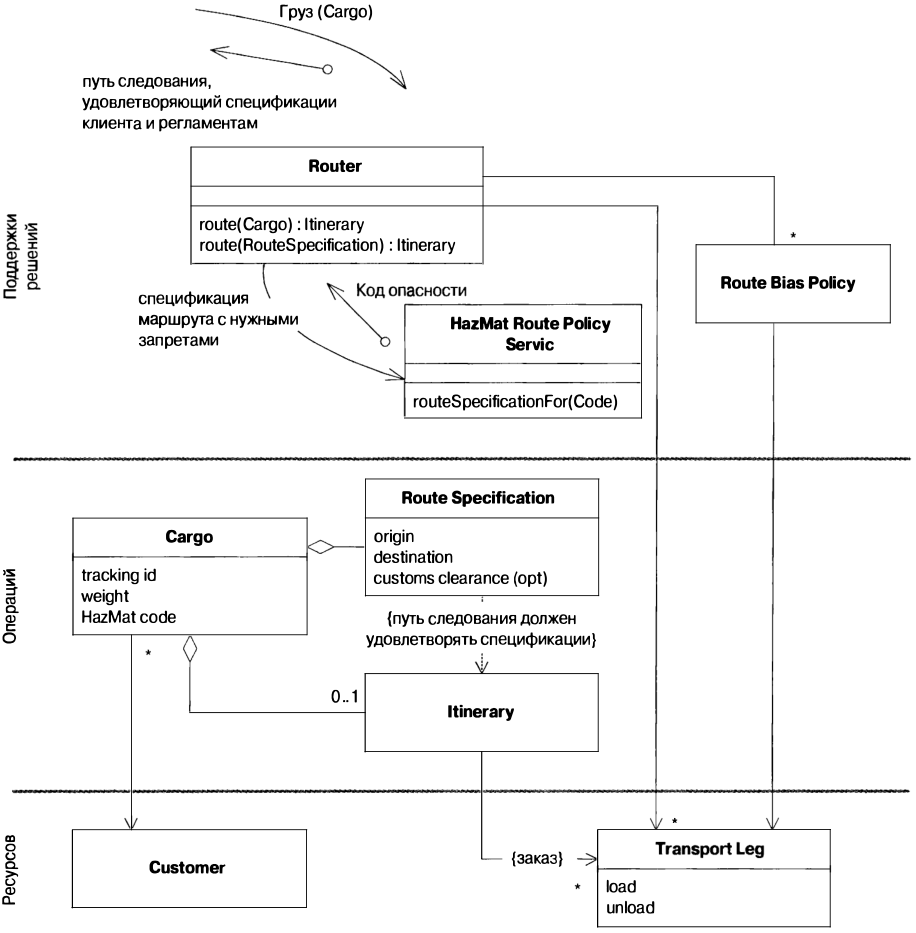
\includegraphics[width=0.8\textwidth]{cargoHazMatOk.png}
\end{center}

И теперь бронирование перевозки выглядит так:

\begin{center}
    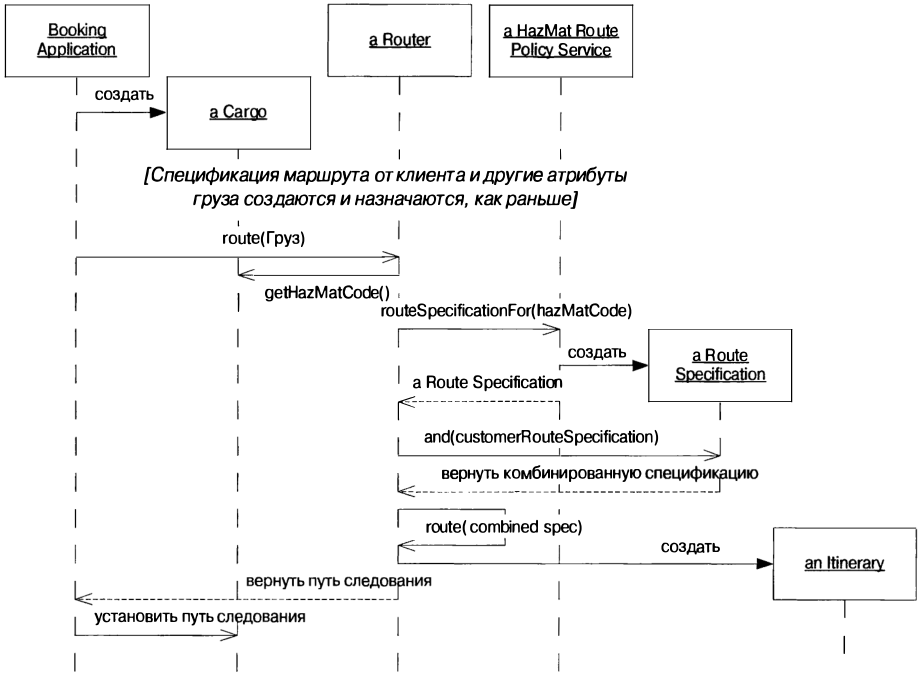
\includegraphics[width=0.9\textwidth]{cargoHazMatOkSequence.png}
\end{center}

Груз теперь ничего про Спецификации маршрута знать не хочет, Маршрутизатор просто принимает Груз, спрашивает его код опасности, формирует по нему Спецификацию маршрута, мерждит её с заказанной Клиентом Спецификацией маршрута, создаёт Расписание и возвращает приложению. Если Клиент доволен, Расписание выставляется Грузу, и вперёд.

Мораль этой истории такова, что крупномасштабная структура имеет приоритет над сиюминутными требованиями, и если требуется рефакторинг для её поддержания, его однозначно стоит провести, вместо того, чтобы легко и быстро реализовать новую функциональность, слегка отклонившись от установленных ограничений. Потому что потом получится архитектурная эрозия, Lava Flow и смерть проекта от собственной сложности.

\subsection{Типичные уровни}

Такое разделение на уровни, которое у нас получилось в примере, на самом деле не случайно и часто встречается в реальных системах в разных вариациях. Например, для систем автоматизации производства типична следующая четырёхуровневая крупномасштабная структура:

\begin{center}
    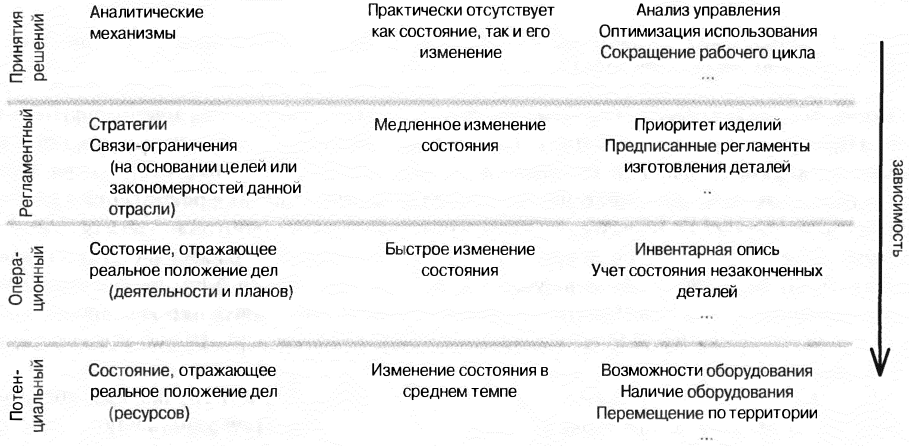
\includegraphics[width=0.9\textwidth]{factoryAutomationLayers.png}
\end{center}

Самый нижний уровень, Потенциальный, как и у нас, отражает наши возможности --- оборудование, производственные площади, контракты с постоянными поставщиками и т.д. Операционный уровень отвечает за оперативное управление --- это конкретно какие детали сейчас есть на складе, статус производства, оперативный план и его выполнение, рабочие на рабочих местах. Регламентный уровень отвечает за ограничения, которых мы должны придерживаться при управлении и планировании --- технические регламенты, законодательство, локальные акты и требования (график отпусков, например), стратегия предприятия. Уровень Принятия решений отвечает за стратегическое управление --- анализ и оптимизацию рабочего цикла.

Каждый уровень имеет разный темп изменения ситуации: потенциальный меняется относительно редко --- оборудование или помещения вряд ли часто меняются в течение одного рабочего дня. Данные на операционном уровне обновляются постоянно. Данные на регламентном уровне обновляются вообще раз в несколько лет. Уровень принятия решений своего состояния как правило вообще не содержит, пользуясь данными, которые предоставляют уровни ниже. Это можно использовать для планирования схемы БД и оптимизации запросов.

Для финансовых систем более типична тоже четырёхуровневая структура, но с другими уровнями:

\begin{center}
    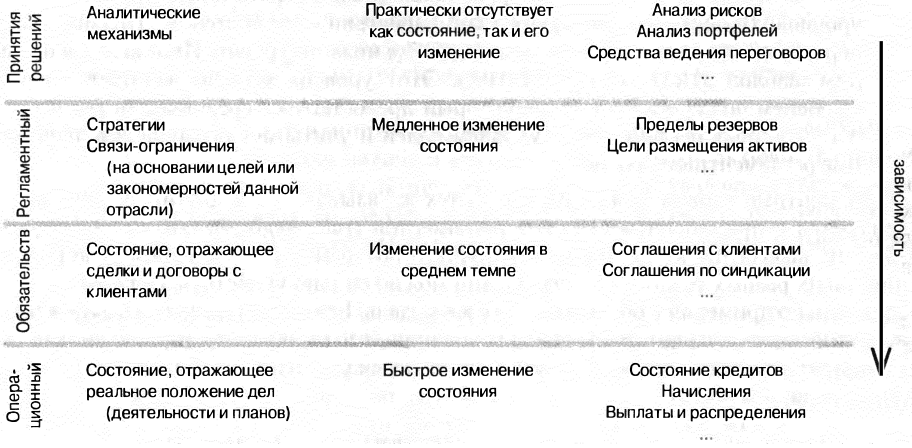
\includegraphics[width=0.9\textwidth]{accountingLayers.png}
\end{center}

Тут Потенциальный уровень отсутствует вообще, потому что финансовые системы не требуют особого оборудования (по крайней мере, того, чем надо реально управлять --- если вы не Сбербанк), они оперируют деньгами. Собственно финансовые операции проводятся на операционном уровне, самом нижнем в такой схеме. Однако добавляется уровень Обязательств --- это на самом деле то, в чём заинтересована финансовая организация и то, что она на самом деле продаёт (например, кредит --- выглядит он так, будто вам продают деньги, но на самом деле это обмен обязательствами). На уровне Обязательств существуют договора, сделки и т.д. Регламентный уровень и уровень Принятия решений имеют тот же смысл и те же особенности, что и для производственных систем.

\subsection{Другие высокоуровневые структуры}

Помимо уровневой, бывают и другие высокоуровневые структуры, причём тысячи их. Например, Подключаемые компоненты (Pluggable Component Framework) --- когда у нас есть ядро системы и плагинная система, которая позволяет динамически подключать/отключать плагины, которые и реализуют большую часть полезной функциональности. На самом деле, большинство современных систем в той или иной степени используют такой подход, кто-то целиком полагаясь на плагины (Visual Studio Code, в каком-то смысле IDEA), кто-то используя их очень ограниченно (например, браузеры --- хотя это зависит от предпочтений пользователя). Даже Linux можно рассматривать как плагинную систему, где есть относительно простое ядро и куча кода, который в него встраивается с помощью чётко определённых интерфейсов.

Ещё интересная структура --- это <<Уровень знаний>>, когда система содержит в себе данные операционного уровня и метаданные (данные о данных) на уровне знаний:

\begin{center}
    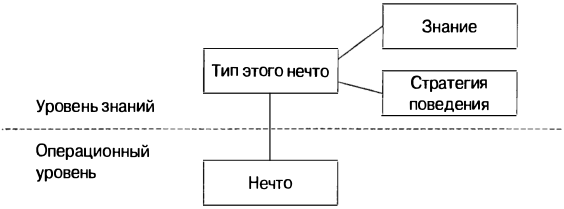
\includegraphics[width=0.65\textwidth]{knowledgeLevel.png}
\end{center}

Уровень знаний --- это обычные объекты в памяти, просто они определяют, что и как можно делать с объектами операционного уровня (например, рефлекция --- на уровне знаний объекты типа Type/Class, на операционном уровне --- обычные объекты). Такой подход мы использовали, естественно, при проектировании систем визуального моделирования и метамоделирования, там правила визуального языка естественно представляются с помощью уровня знаний, который можно редактировать даже прямо во время выполнения, от чего операционный уровень начинает вести себя по-другому. 

В финансовых системах такой подход позволяет на уровень знаний вынести финансовые продукты --- например, хитрые правила начисления процентов по вкладам, которые постоянно меняются и реализовывать их в коде было бы весьма неразумно. Регламенты с уровня знаний там затем применяются к финансовым потокам на операционном уровне, при этом система становися очень гибкой --- при наличии годного редактора правила может менять даже финансист, который программировать вообще не умеет. Конечно, у такого подхода есть и недостаток --- логика уровня знаний не проверяется компилятором и имеет ту семантику, которую криворукие программисты реализуют, так что чрезмерное увлечение такими делами (когда у вас вся система представляется в виде правил на XML, например) может превратить поддержку в настоящий кошмар.

И последняя мысль по поводу крупномасштабной структуры --- это то, что крупномасштабная структура для системы одна, но разные архитектурные стили не исключают друг друга, и, например, можно использовать уровневую структуру для системы в целом и <<Уровень знаний>> для реализации какого-нибудь из уровней, а плагины --- для какого-то другого.

\end{document}